% !Mode:: "TeX:UTF-8"

\chapter{绪~~论}
\section{引言}

从1931年Ernst Ruska制造了世界上第一台电子显微镜(图1.1a)~\cite{das1932}至今,人类的显微镜分辨率以前所未有的速度提升(图1.1b)。球差矫正器的发明~\cite{dev1997}更是将透射电子显微镜(transmission electron microscopy,TEM)的分辨率提升至亚埃级别,使人类具备了观察原子的常规手段。TEM在众多学科中都发挥了关键的作用,其模式和功能日益多样化,成像理论日益完善和成熟。 

\begin{figure}[htbp]
	\vspace{\baselineskip}
	\centering
	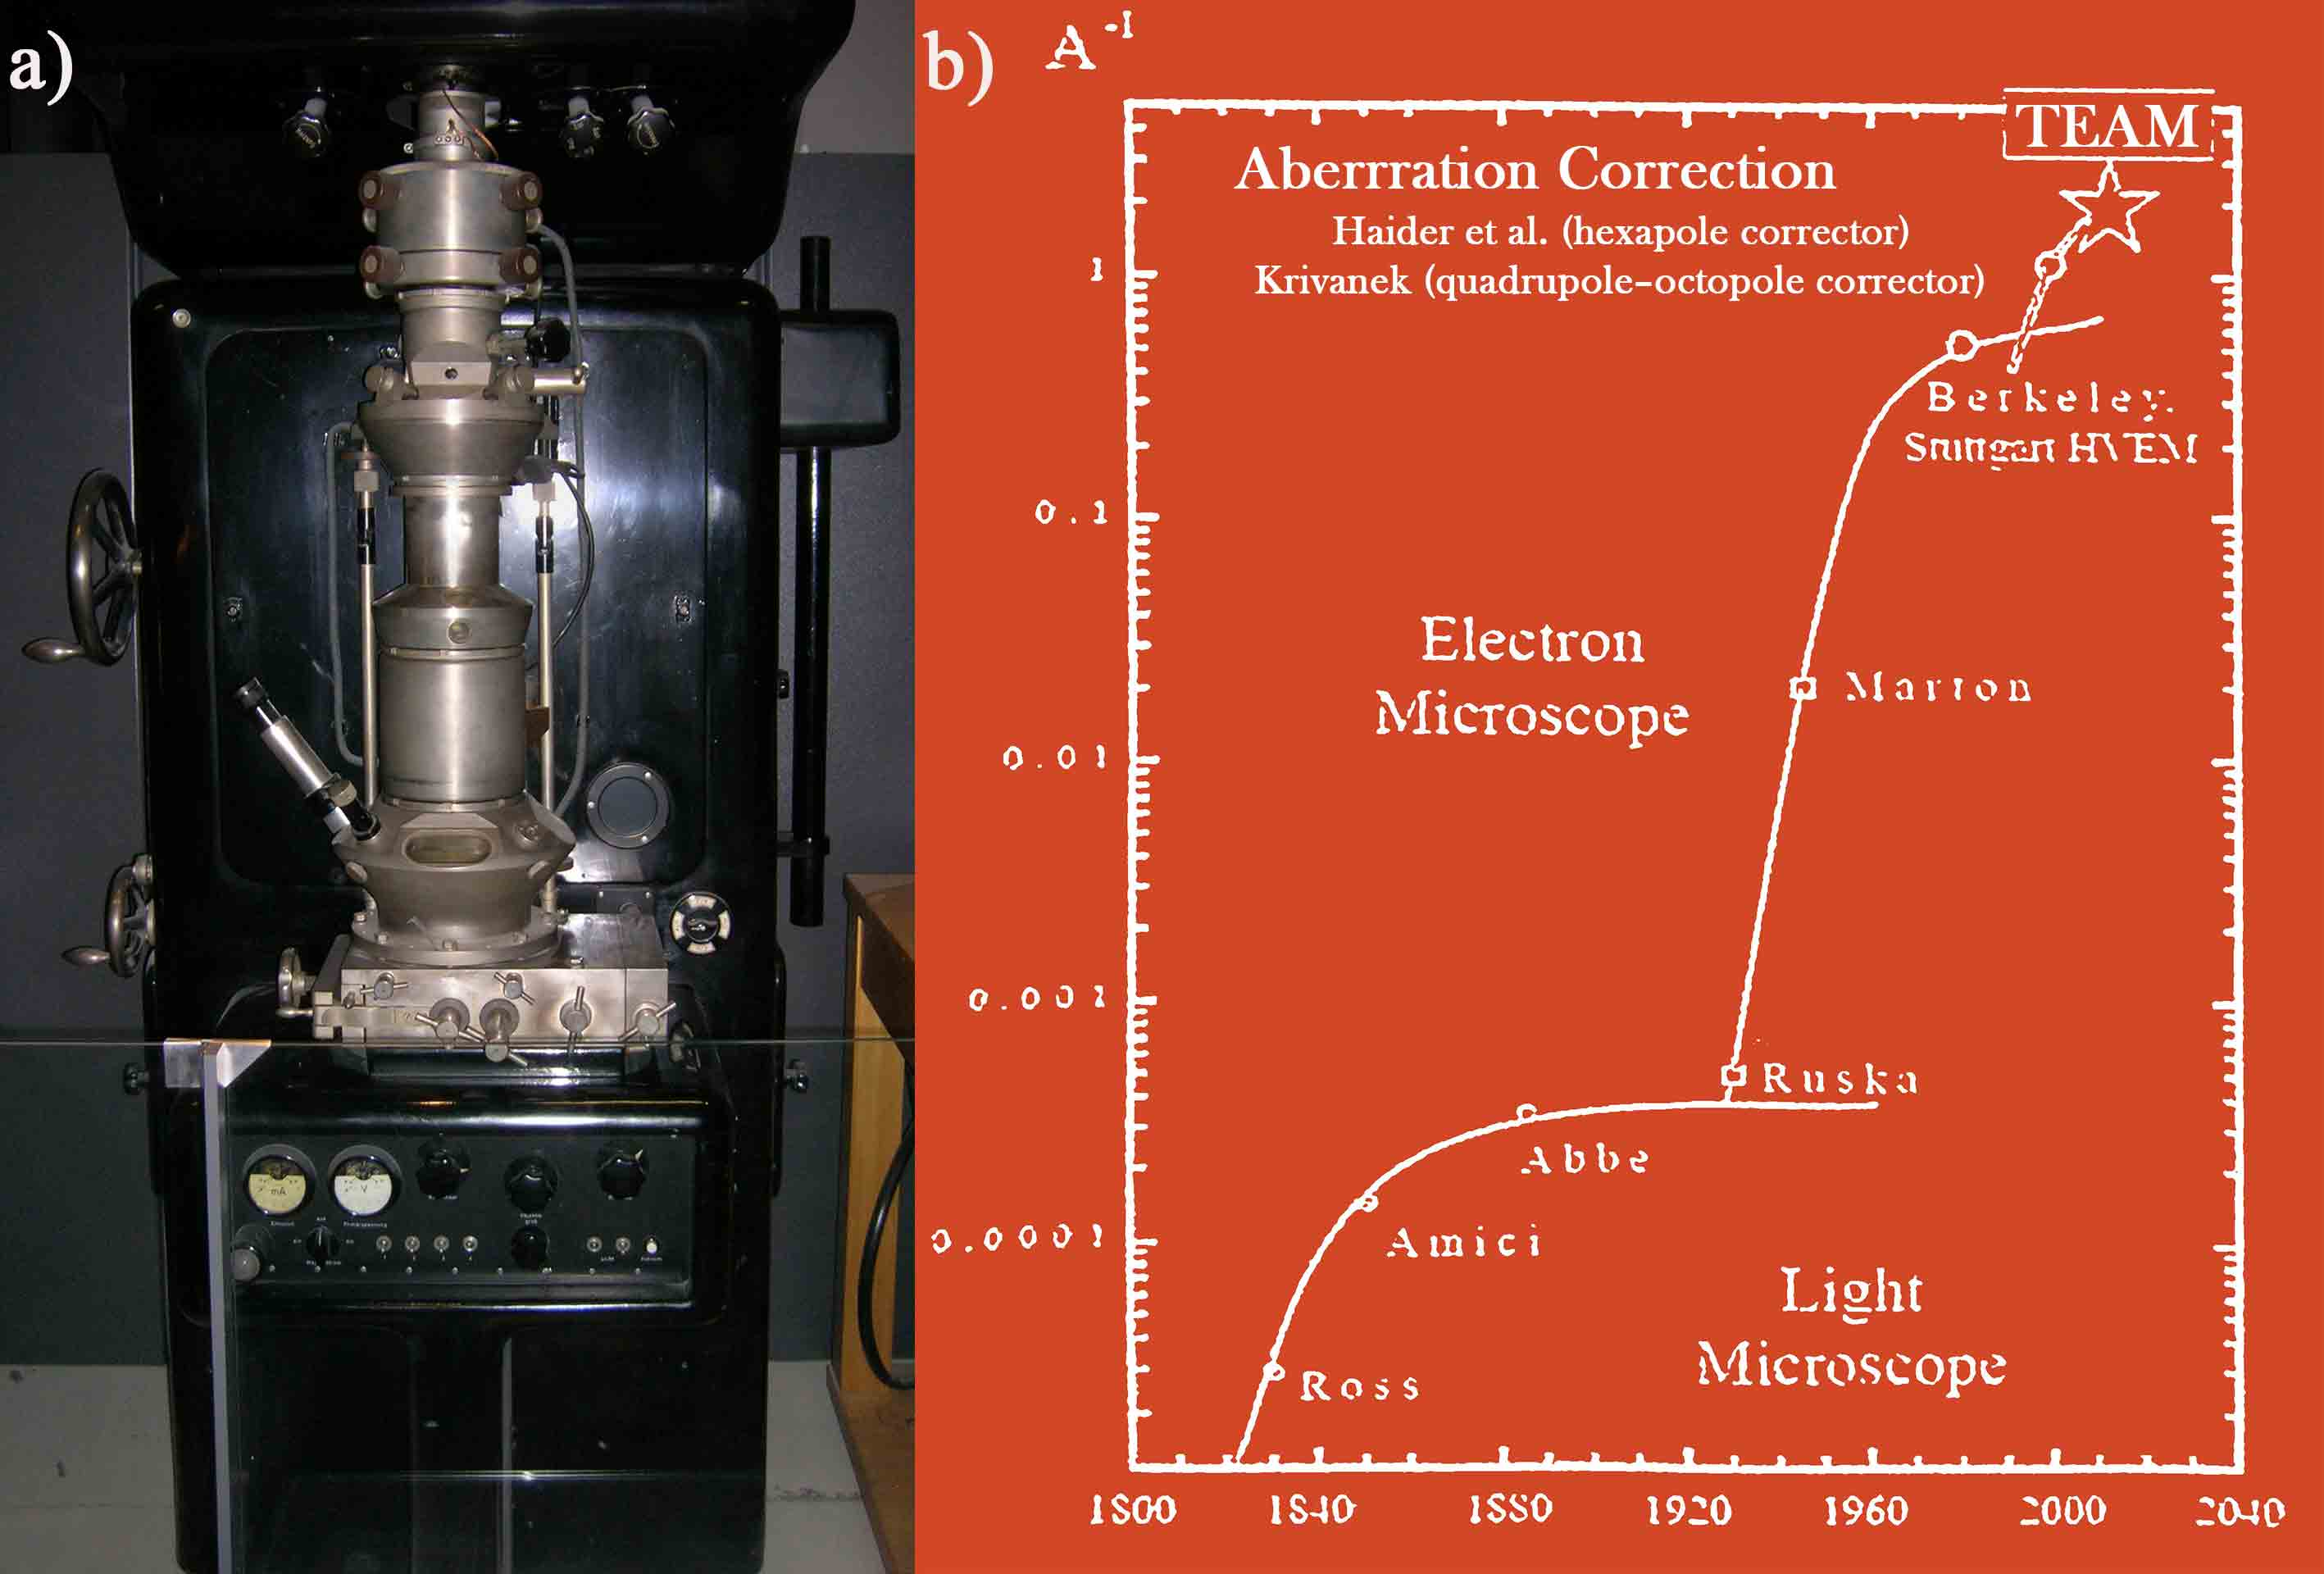
\includegraphics[width=0.8\textwidth]{../1.1/11}
	\caption{世界上第一台电子显微镜与显微镜分辨率发展曲线}\label{fig:11}
	\song\wuhao{a) 世界上第一台电子显微镜;b) 显微镜分辨率发展曲线}
\end{figure}

材料的三维结构对其宏观性能具有很重要的影响。比如铝合金中的析出相的形貌、尺寸以及分布决定其析出强化的效果;纳米颗粒的形貌和尺寸会影响其催化性能、分布状况等。获取材料的三维结构、成分、分布等信息,而不仅仅是二维投影信息,是材料科学研究中一个极其重要的问题。TEM在材料科学领域的应用已经相当广泛,其各种二维原子成像手段更是具有不可替代的作用。TEM在获取材料三维信息方面也具有很多的应用,其手段也是多种多样。三维电子断层扫描[3-7](three-dimensional electron tomography,3DET)技术是应用最广泛的三维重构技术,其基本理论与医学电子计算机断层扫描(computed tomography,CT)的理论相同,通过收集物体多个方向的投影来恢复出物体内部的三维信息。扫描透射电子显微镜(scanning transmission electron microscopy,STEM)以及高角环形暗场(high angle annular dark field,HAADF)成像模式的发明,普及了3DET技术的应用[8-11],并使其能够达到原子分辨率。STEM分辨率的不断提升,还催生了光学层析[10, 12-17]三维重构的运用。但是,这两种三维重构的方法,依然面对着种种问题限制着它们的应用,比如缺失锥[18-25]、辐照损伤[26]、样品漂移[27-30]等等。